\chapter{Conceptual Design}
Ein erstes Design für die Benutzeroberfläche wird mit einem Mockup Tool entwickelt. Hierbei geht es primär darum Unstimmigkeiten und grobe Fehleinschätzungen auszumerzen, um anschließend einen funktionalen Prototypen zu entwickeln.

\subsubsection*{Mockups}
\begin{figure}[ht]
\centering
\begin{minipage}[b]{.5\textwidth}
  \centering
  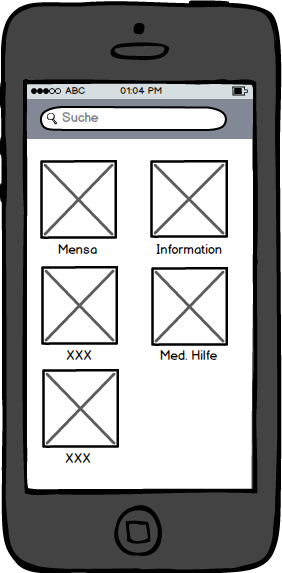
\includegraphics[width=.8\linewidth]{img/menu-mockup.png}
  \label{img:menu-mockup}
  \captionof{figure}{Menü Mockup}
\end{minipage}%
\begin{minipage}[b]{.5\textwidth}
  \centering
  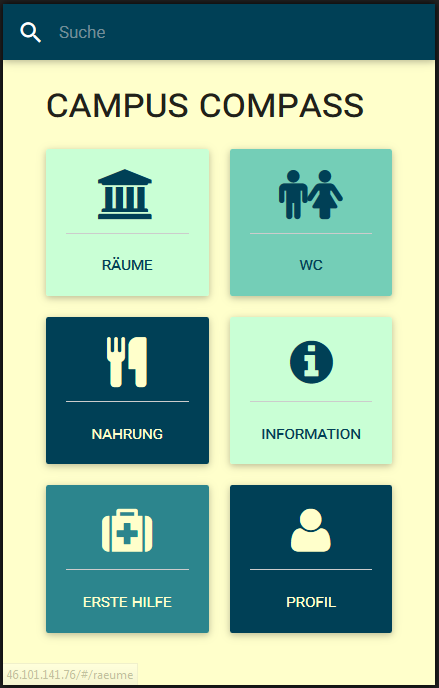
\includegraphics[width=.8\linewidth]{img/menu.png}
  \label{img:menu-first-draft}
  \captionof{figure}{Erster Entwurf Menü}
\end{minipage}
\end{figure}

\begin{figure}[ht]
\centering
\begin{minipage}[b]{.5\textwidth}
  \centering
  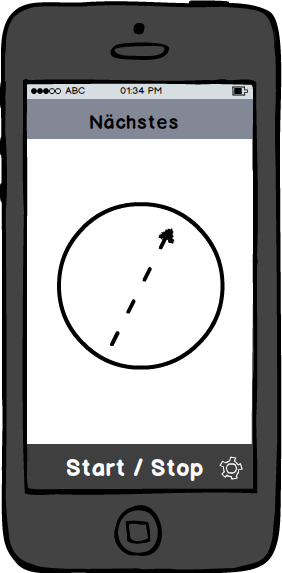
\includegraphics[width=.8\linewidth]{img/navigation-mockup.png}
  \label{img:navigation-mockup}
  \captionof{figure}{Navigation Mockup}
\end{minipage}%
\begin{minipage}[b]{.5\textwidth}
  \centering
  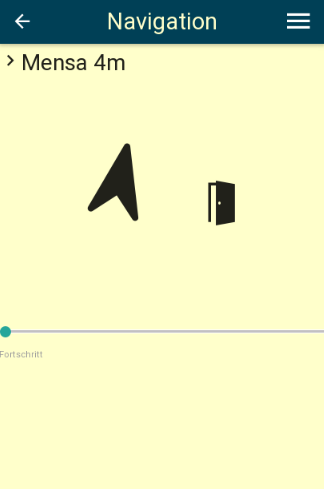
\includegraphics[width=.8\linewidth]{img/navigation.png}
  \label{img:navigation-first-draft}
  \captionof{figure}{Erster Entwurf Navigation}
\end{minipage}
\end{figure}

\begin{figure}[ht]
\centering
\begin{minipage}[b]{.5\textwidth}
  \centering
  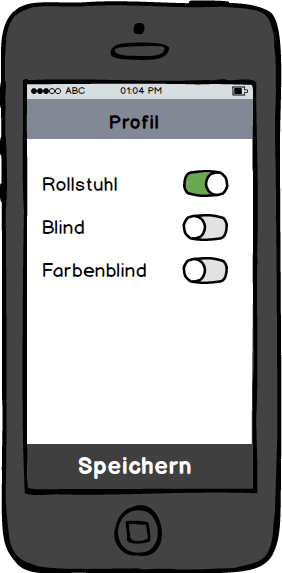
\includegraphics[width=.8\linewidth]{img/profil-mockup.png}
  \label{img:profil-mockup}
  \captionof{figure}{Profil Mockup}
\end{minipage}%
\begin{minipage}[b]{.5\textwidth}
  \centering
  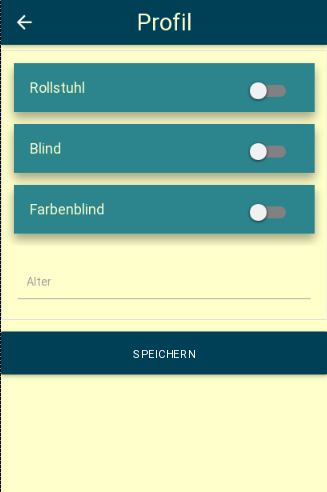
\includegraphics[width=.8\linewidth]{img/profil.png}
  \label{img:profil-first-draft}
  \captionof{figure}{Erster Entwurf Profil}
\end{minipage}
\end{figure}

\begin{figure}[ht]
\centering
\begin{minipage}[b]{.5\textwidth}
  \centering
  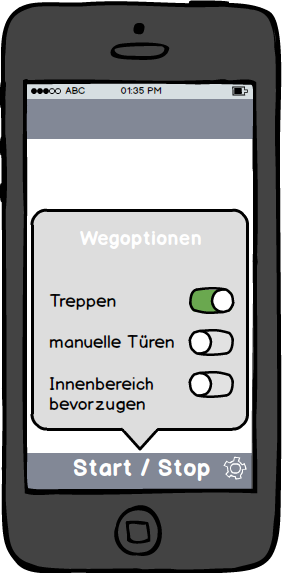
\includegraphics[width=.8\linewidth]{img/wegoptionen-mockup.png}
  \label{img:wegoptionen-mockup}
  \captionof{figure}{Wegoptionen Mockup}
\end{minipage}%
\begin{minipage}[b]{.5\textwidth}
  \centering
  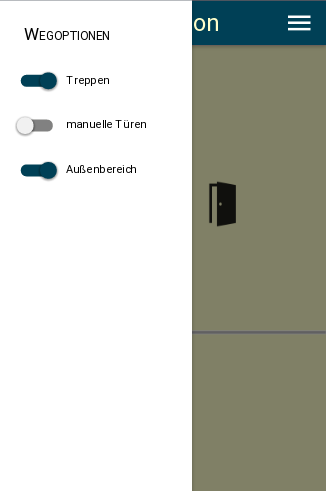
\includegraphics[width=.8\linewidth]{img/wegoptionen.png}
  \label{img:wegoptionen-first-draft}
  \captionof{figure}{Erster Entwurf Wegoptionen}
\end{minipage}
\end{figure}